\documentclass[a4paper]{article}

\usepackage[utf8]{inputenc}
\usepackage[margin=2cm, top=2cm, includefoot]{geometry}
\usepackage[english]{babel}
\usepackage{graphicx}
\usepackage[table, xcdraw]{xcolor}
\usepackage{fancyhdr}
\usepackage[most]{tcolorbox}
\usepackage[hidelinks]{hyperref}
\usepackage{parskip}
\usepackage{smartdiagram}
\usepackage{listings}
\usepackage{zed-csp}


\setlength{\headheight}{40.2pt}
\pagestyle{fancy}
\fancyhf[]{}
\newcommand{\sectionName}{Contents}

% adding images over the fancy line
%\lhead{\includegraphics[]{}}
\rhead{\sectionName}

\renewcommand{\headrulewidth}{3pt}

% Adding code into the document
\lstdefinestyle{mystyle}{
    backgroundcolor=\color{backcolour},   
    commentstyle=\color{codegreen},
    keywordstyle=\color{magenta},
    numberstyle=\tiny\color{codegray},
    stringstyle=\color{codepurple},
    basicstyle=\ttfamily\footnotesize,
    breakatwhitespace=false,         
    breaklines=true,                 
    captionpos=b,                    
    keepspaces=true,                 
    numbers=left,                    
    numbersep=5pt,                  
    showspaces=false,                
    showstringspaces=false,
    showtabs=false,                  
    tabsize=2
}

\renewcommand{\lstlistingname}{Code} % Chaning the caption name where code appears
\lstset{style=mystyle}

\newcommand\tab[1][1cm]{\hspace*{#1}}

% Declaration of colors 
\definecolor{codegreen}{rgb}{0,0.6,0}
\definecolor{codegray}{rgb}{0.5,0.5,0.5}
\definecolor{codepurple}{rgb}{0.58,0,0.82}
\definecolor{backcolour}{rgb}{0.95,0.95,0.92}

%Bibliography
%\bibliographystyle{plain}


\begin{document}
    \cfoot{\thepage}
    \begin{titlepage}
        \centering
        \vfill
        {\huge\bfseries{Virtual Machines}} \par
        \vspace{0.2cm}
        {\LARGE{\textbf{Explanation and Guide}}} \par
        \vfill
        {
            \large{
                \textit{Sergio Miguez Aparicio} \par
                \textit{December 2021} \par
                }
        }
        \vfill
        
    \end{titlepage}


%___________________________________________________________________________________________________________
    \clearpage 
    \tableofcontents

%___________________________________________________________________________________________________________
    \clearpage
    \section{\textbf{Introduction}}
    \renewcommand{\sectionName}{Introduction}
    \tab A Virtual Machine (VM) is a computer that runs over software instead of physical computing resources.
    The system can operate full independent inside the "host" machine running programs, and processes in the
    the same way a normal computer would do.

    \tab A Virtual Machine will run an OS, which could be of any type and version. Some examples would be 
    Windows 10/11/7/XP, a Linux distribution (Arch, Ubuntu, Parrot OS, Linux Mint, etc).

    \vspace{0.5cm}
    \subsection{Benefits and Disadvantages}
    
    \tab The \textbf{benefits} of using VMs are:
    \begin{enumerate}
        \item Allows running full operating systems.
        \item Dedicating the specific resources that a process will need.
        \item Testing and running processes in safe environments (sandboxes).
        \item Can run multiple OS environments in the same computer.
        \item Support legacy applications, reducing migration cost from one OS to another.
        \item Regardless of the main host system, a VM can run any OS without compatibility issues.
    \end{enumerate}
    
    \vspace{0.5cm}

    \tab Some \textbf{disadvantages} are:
    \begin{enumerate}
        \item It is hardware expensive to run multiple Virtual Machines simultaneously.
        \item They are less efficient and are slower than a full physical computer.
    \end{enumerate}

    \vspace{0.5cm}

    \subsection{Types of Virtual Machines}
    \tab There are \textbf{two different types} of Virtual Machines:
    \vspace{0.35cm}

    \begin{center}
        \smartdiagram[descriptive diagram]{
            {Process Virtual Machine,{allows a single process to run in a separate virtualized
                    environment.}},
            {System Virtual Machine, {Full virtualized system to emulate a physical machine.
                    Host resources are shared with the VM.}},
        }
    \end{center}

    \vspace{0.5cm}
    \subsection{Types of Virtualization}
    \tab There are \textbf{5 types of virtualization}:

    \vspace{0.15cm}

    \begin{enumerate}
        \item Hardware Virtualization: also known as server virtualization, allows using hardware resources
            efficiently to run multiple VMs at the same time. The hardware is not allocated and
            managed between the different systems.
        \item Software Virtualization: creates a full computer with dedicated hardware to run an OS.
        \item Storage Virtualization: join different storage hardware resources to appear as a single unit.
            It increases performance, data management, reduction of downtime and transfer of data
        \item Network Virtualization: creating multiple separated networks from a unique physical one.
           Bandwidth can be allocated, improving reliability, security and monitoring.
        \item Desktop Virtualization: separates the desktop from the physical device. It is accessed remotedly
            allowing users to access their working environment wherever they want.
    \end{enumerate}

    \subsection{Difference between a VM and a Container}

    \tab Containers allow running isolated applications on a platform. It is in this way that is similar to 
    Virtual Machines. The key aspect which differentiates them is that a VM will virtualize the hardware, creating 
    a full computer, while the container will include the process and its dependencies to run.
    A container shares OS services and focuses on isolating the process through virtual-memory hardware.

    \tab A container is faster and only contains the files required to run the process, being simpler and smaller.
    These characteristics benefit using resources, booting faster and delivering applications easier.

    \tab On the other side, VMs are larger and slower. They have their independent OS kernel and offer the benefits
    of a completely isolated system. 


%___________________________________________________________________________________________________________
    \clearpage
    \section{Setting up your Linux Machine}
    \renewcommand{\sectionName}{Setting up your Linux Machine}
    \tab In this section, I will be using a Virtual Machine (VM) with Parrot OS, version 4.11.3. This machine 
    was previously set up, but in order of completion, I will cover how to create your own Parro VM.

    \tab There are multiple programs that can be used. I have previously used \href{https://www.vmware.com/}
    {\textcolor{blue}{\textit{VMware (free license)}}} and \href{https://www.virtualbox.org/}{\textcolor{blue}{\textit{Oracle VM VirtualBox
    (free license)}}}. Both have pretty similar configuration options, so feel free to use the one you like the most. I 
    will be using \href{https://www.vmware.com/products/workstation-player/workstation-player-evaluation.html}
    {\textcolor{blue}{\textit{VMware Workstation 16 (free license)}}} 

    \subsection{\textbf{Installing WMware Workstation 16 Pro in Windows}}
    \begin{enumerate}
        \item Download the installer from the website previously provided.
        \item Execute it with administrator permisions.
        \item Install using the following configurations
    \end{enumerate}

    \vfill

    \begin{tcolorbox}[colback=red!5!white,colframe=red!75!black]
        \centering
        \textbf{
        The Pro version is not free, but the software includes the "VMware Workstation 16 Player", which can be
        used with a free license. You can install instead  "VMware Workstation 16" (not Pro). This other version will only
        include the Player software. The steps to get it installed are exactly the same.
        }
    \end{tcolorbox}

    \vfill

    \begin{figure}[h]
        \centering
        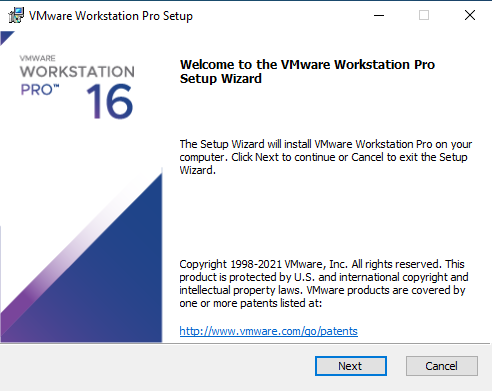
\includegraphics[width=0.7\textwidth]{Images/Install_VMware/Install_VMware_1.png}
        \caption{Press "Next".}    
    \end{figure}

    \vfill
%___________________________________________________________________________________________________________
    \clearpage    
    \begin{figure}
        \centering
        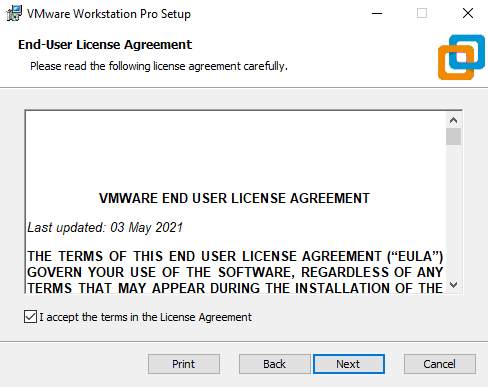
\includegraphics[width=0.7\textwidth]{Images/Install_VMware/Install_VMware_2.png}
        \caption{Accept the terms and Press "Next".}    
    \end{figure}

    \vfill

    \begin{figure}
        \centering
        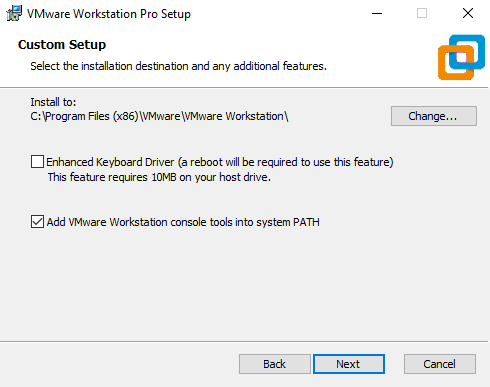
\includegraphics[width=0.7\textwidth]{Images/Install_VMware/Install_VMware_3.png}
        \caption{Tick add VMware to PATH and Press "Next".}    
    \end{figure}
%___________________________________________________________________________________________________________
    \clearpage    
    \begin{figure}
        \centering
        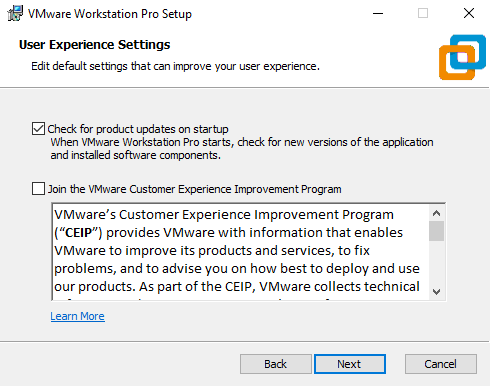
\includegraphics[width=0.7\textwidth]{Images/Install_VMware/Install_VMware_4.png}
        \caption{Un tick joining the Customer Experience Improvement Program and Press "Next".}    
    \end{figure}

    \vfill

    \begin{figure}
        \centering
        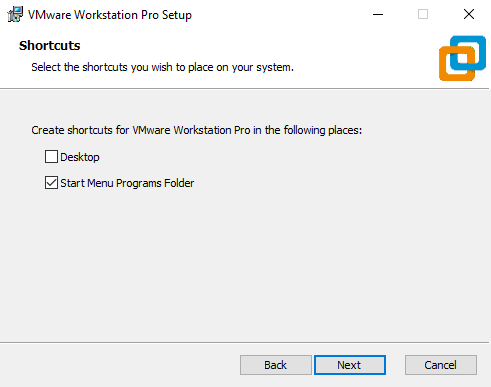
\includegraphics[width=0.7\textwidth]{Images/Install_VMware/Install_VMware_5.png}
        \caption{Press "Next".}   
    \end{figure}
    
%___________________________________________________________________________________________________________
    \clearpage
    \begin{figure}
        \centering
        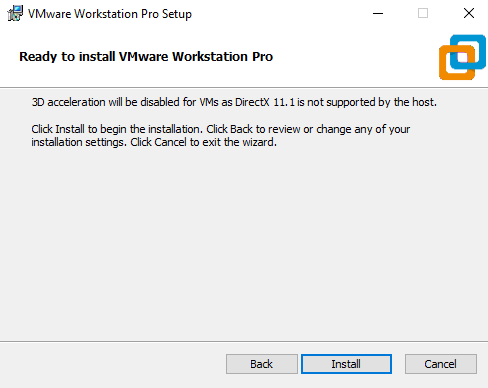
\includegraphics[width=0.7\textwidth]{Images/Install_VMware/Install_VMware_6.png}
        \caption{Press "Install".}    
    \end{figure}

    \vfill

    \begin{figure}
        \centering
        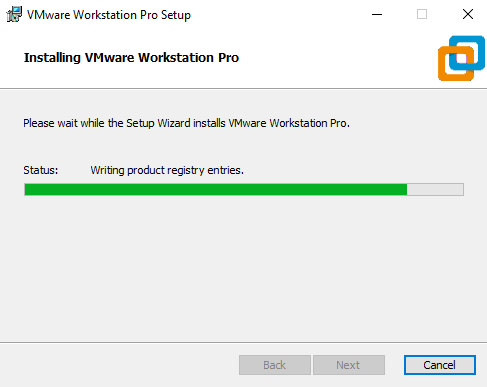
\includegraphics[width=0.7\textwidth]{Images/Install_VMware/Install_VMware_7.png}
        \caption{Wait while installing.}    
    \end{figure}

%___________________________________________________________________________________________________________
    \clearpage
    \begin{figure}[h]
        \centering
        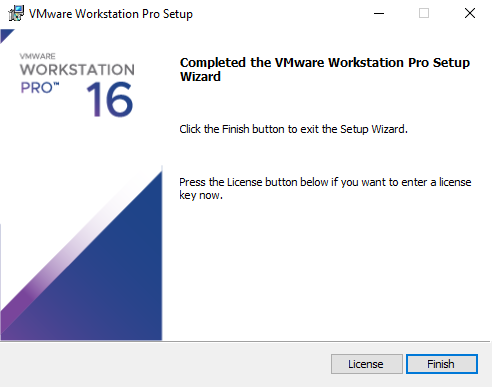
\includegraphics[width=0.7\textwidth]{Images/Install_VMware/Install_VMware_8.png}
        \caption{The instalation has finished, press "Finish".}                
    \end{figure}

    \vspace{1cm}

    \begin{tcolorbox}[colback=green!5!white,colframe=green!75!black]
        \centering
        \textbf{Completed all these previous steps, you will correctly have installed the VMware Workstation Pro 16 software.}
    \end{tcolorbox}

    \vspace{1.5cm}

    \subsection{\textbf{Creating a VM in VMware Workstation 16 Player}}
    \tab To create a new Virtual Machine, you will need to download the ISO of the Linux Distribution you want
    to use. As previously mentioned, we will be using Parrot OS. You can download it using the following \href
    {https://www.parrotsec.org/download/}{\textcolor{blue}{\textit{link}}}.
    The version of Parrot OS that I will be using is the MATE Parrot OS 4.11.3.
    Feel free to install the distribution you want. Ubuntu, Parrot, Linux Mint. Most of them have a 
    pretty similar installation. The process of creating the Virtual Machine will be exactly the same for all
    of them as it is independent of the OS (just to VMware).

%___________________________________________________________________________________________________________
    \clearpage

    \begin{figure}[h]
        \centering
        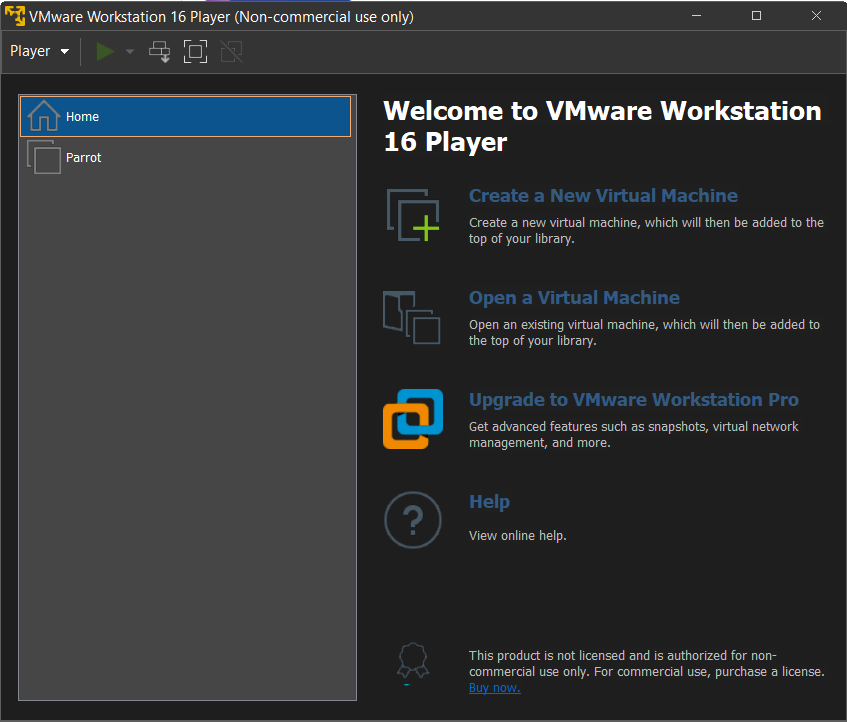
\includegraphics[width=0.7\textwidth]{Images/Create_VM/Creating_VM_1.png}
        \caption{Press "Create a New Virtual Machine"}
    \end{figure}

    \vfill

    \begin{figure}[h!]
        \centering
        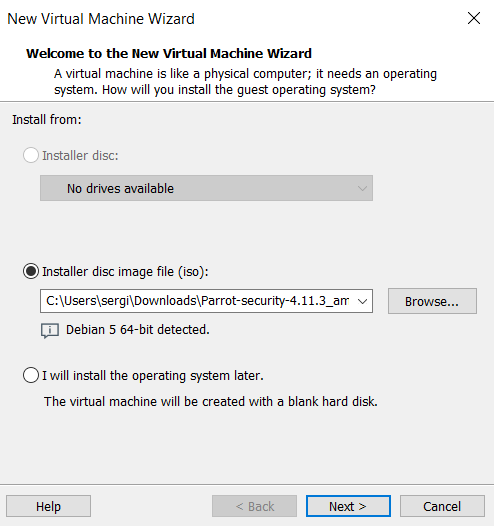
\includegraphics[height=11cm, keepaspectratio]{Images/Create_VM/Creating_VM_2.png}
        \caption{Select the 2\textsuperscript{nd} option, Browse and Select the ISO you previously downloaded. Then, press "Next".}
    \end{figure}

%___________________________________________________________________________________________________________
    \clearpage

    \begin{figure}[h]
        \centering
        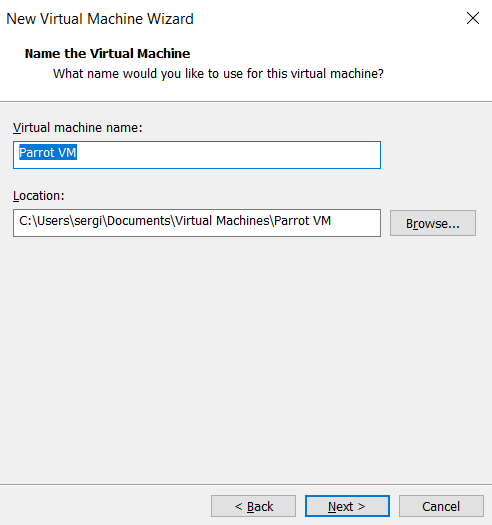
\includegraphics[height=10cm, keepaspectratio]{Images/Create_VM/Creating_VM_3.png}
        \caption{Give your Virtual Machine a Name and select the location where you want it to be stored.}
    \end{figure}

    \vfill

    \begin{figure}[h!]
        \centering
        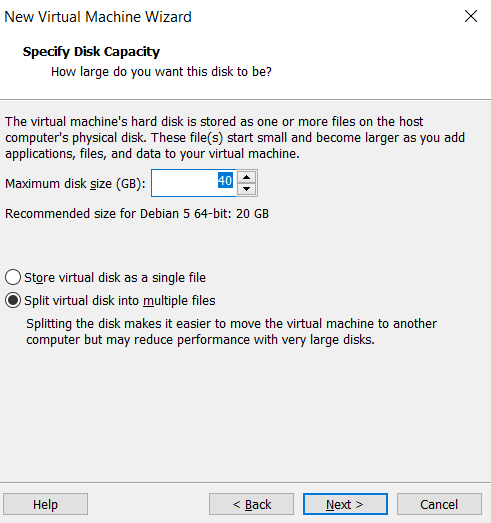
\includegraphics[height=10cm, keepaspectratio]{Images/Create_VM/Creating_VM_4.png}
        \caption{Select the size of the memory of your VM, 40GB is usually more than enough. Press "Next".}
    \end{figure}

%___________________________________________________________________________________________________________
    \clearpage
    \begin{figure}[h]
        \centering
        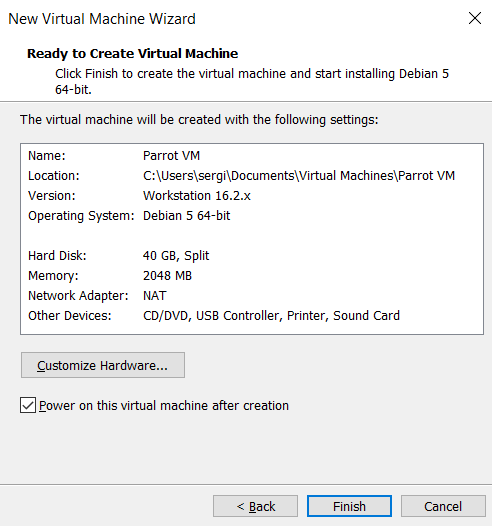
\includegraphics[height=10cm, keepaspectratio]{Images/Create_VM/Creating_VM_5.png}
        \caption{We recommend now Customizing the Hardware, Press "Customize Hardware...", else Press "Finish".}
    \end{figure}

%___________________________________________________________________________________________________________
    \clearpage
    \begin{tcolorbox}[colback=green!5!white,colframe=green!75!black]
        \centering
        \textbf{If you pressed "Customize Hardware", use the following recommendaitons:}
    \end{tcolorbox}

    \vspace{0.5cm}

    \begin{figure} [h]
        \centering
        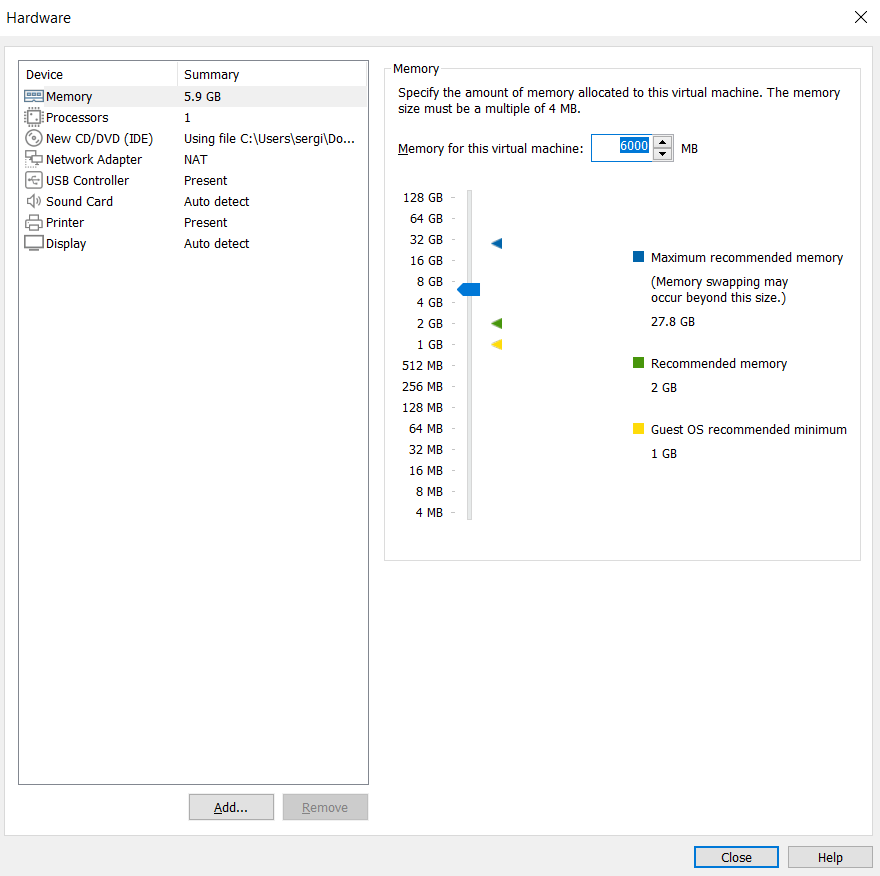
\includegraphics[width=\textwidth, keepaspectratio]{Images/Create_VM/Creating_VM_6.png}
        \caption{Give your VM the RAM memory you want. (Depends on your Hardware specifications which limits the RAM).
        4GB is enough, but I usually go with 6GB.}    
    \end{figure}

    \vspace{0.5cm}

    \begin{tcolorbox}[colback=red!5!white,colframe=red!75!black]
        \centering
        \textbf{Not dedicated enough RAM, the system will go slow, and some applications might collapse.}
    \end{tcolorbox}

%___________________________________________________________________________________________________________
    \clearpage
    \begin{figure} [h]
        \centering
        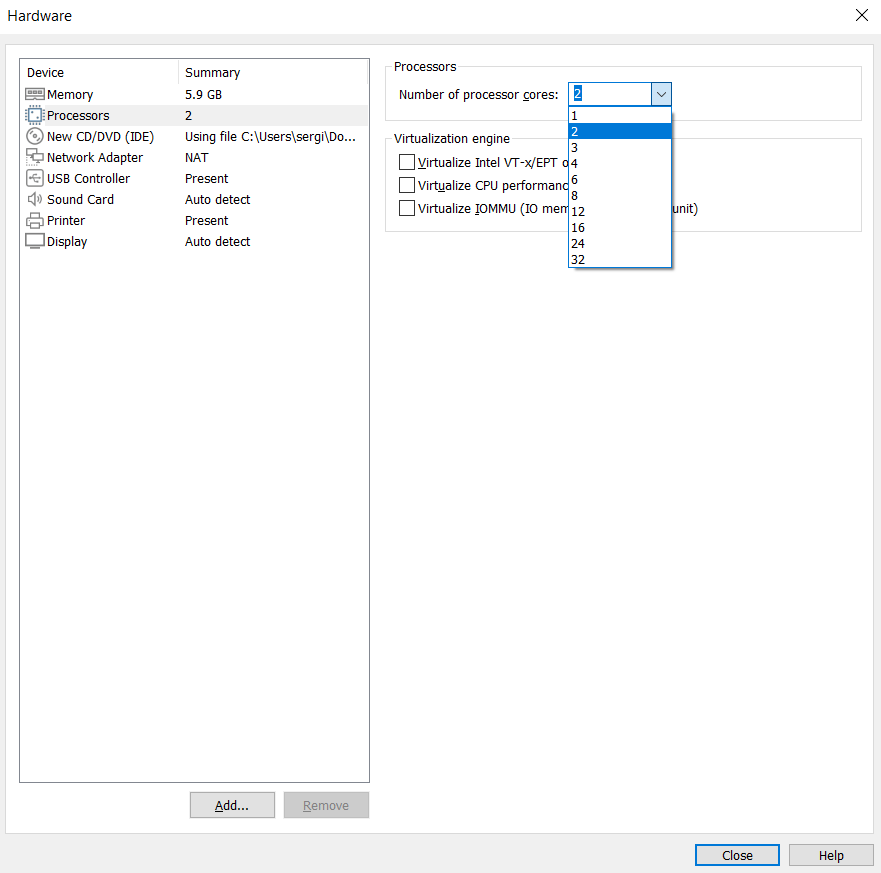
\includegraphics[width=\textwidth, keepaspectratio]{Images/Create_VM/Creating_VM_7.png}
        \caption{Select the number of processor cores for your VM. 1 is usually enough, but more
        will make the machine work faster. I will select 2.}
    \end{figure}

    \vspace{0.5cm}

    \tab Other configurations, such as Network Adapters, Sound Card or Display, can be found in this Panel.
    The Configuration Panel of the VM will be accessible later on too. 

    \vfill

    \begin{tcolorbox}[colback=green!5!white,colframe=green!75!black]
        \centering
        \textbf{Having completed all these steps, your VM will be ready to start running.}
    \end{tcolorbox}

    \vfill
%___________________________________________________________________________________________________________
    \clearpage
    \subsection{\textbf{Installing the Parrot OS}}
    \tab After pressing the "Finish" button in the Configuration Panel, the VM will start immediately. The 
    the system will show the following screen:
    \vspace{0.5cm}
    \begin{figure}[h]
        \centering 
        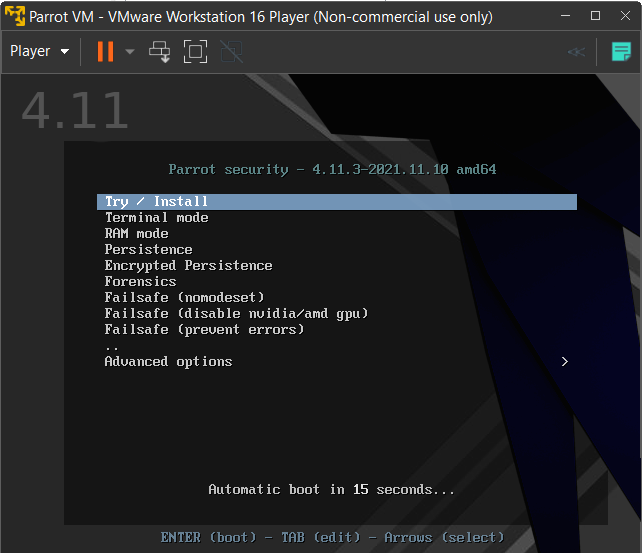
\includegraphics[width=\textwidth, keepaspectratio]{Images/Install_OS/OS_1.png}
        \caption{Press "Enter" in "Try / Install". The system will boot. Other options can be selected, but this 
        will be more than enough for us. This option will let the user try the OS and install it. If any key from the keyboard
        is pressed within 30 seconds, the highlighted option will be selected.}
    \end{figure}

%___________________________________________________________________________________________________________  
    \clearpage
    \begin{figure}[h]
        \centering 
        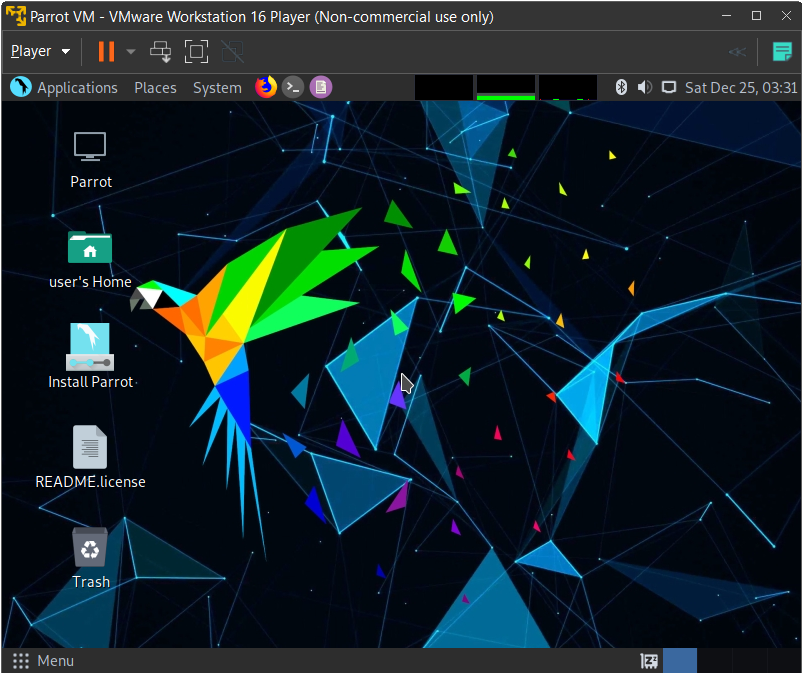
\includegraphics[width=\textwidth, keepaspectratio]{Images/Install_OS/OS_2.png}
        \caption{Parrot OS will launch in a testing mode. You will have full access to try the OS before installing.}
    \end{figure}

    \vfill

    \begin{tcolorbox}[colback=blue!5!white,colframe=blue!75!black]
        \centering
        \textbf{To INSTALL, open the "Install Parrot" icon (double clink) from the Desktop.}
    \end{tcolorbox}

    \vfill

%___________________________________________________________________________________________________________  
    \clearpage
    \begin{figure}[h]
        \centering
        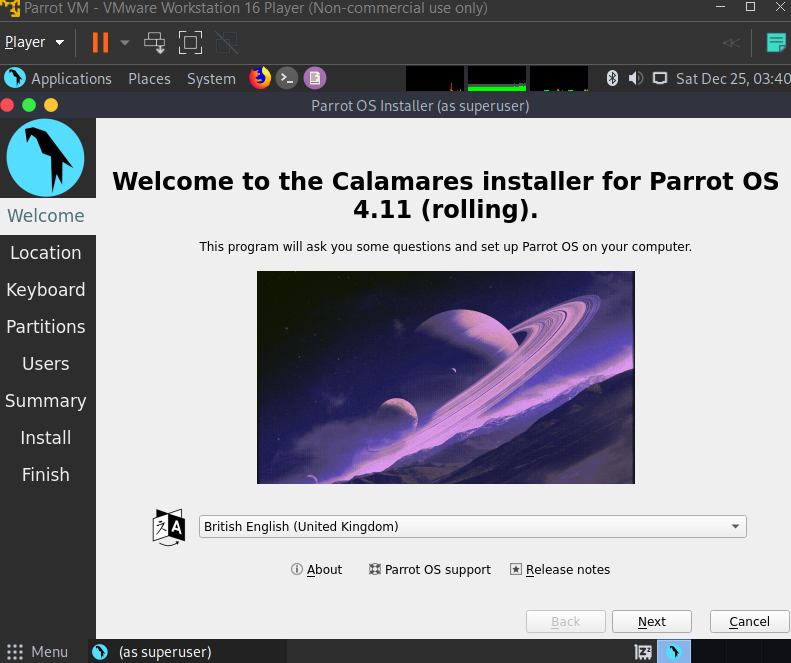
\includegraphics[width=0.75\textwidth]{Images/Install_OS/OS_3.png}
        \caption{Select the language you want to install for your OS and press "Next".}
    \end{figure}

    \vfill

    \begin{figure}[h!]
        \centering
        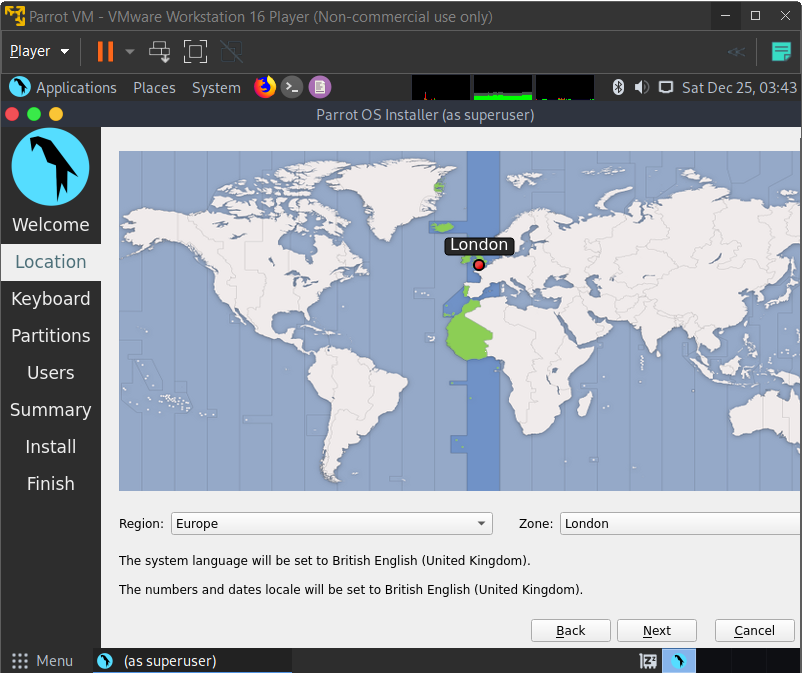
\includegraphics[width=0.75\textwidth]{Images/Install_OS/OS_4.png}
        \caption{Select the timezone of your machine and press "Next".}
    \end{figure}

%___________________________________________________________________________________________________________  
    \clearpage
    \begin{figure}[h]
        \centering
        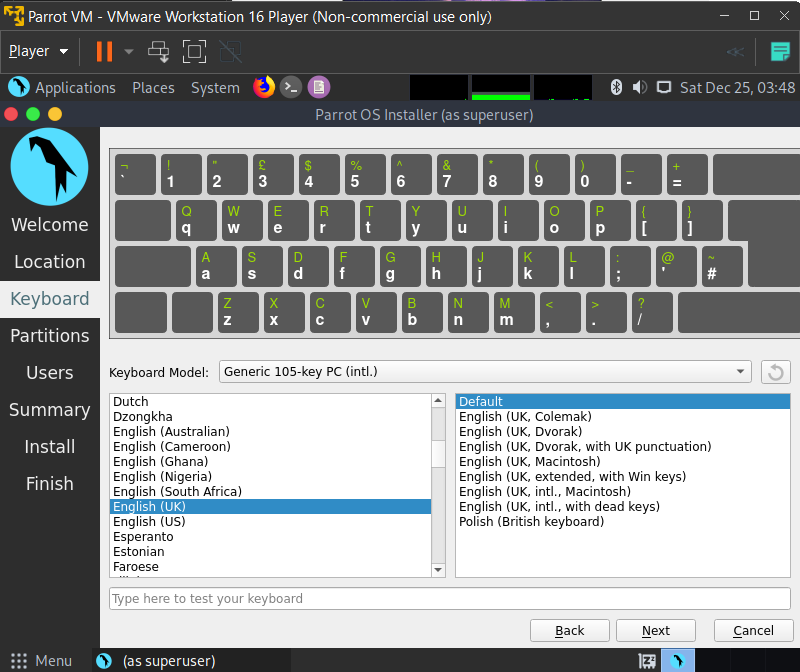
\includegraphics[width=0.75\textwidth]{Images/Install_OS/OS_5.png}
        \caption{Select your keyboard distribuition and press "Next".}
    \end{figure}

    \vfill

    \begin{figure}[h!]
        \centering
        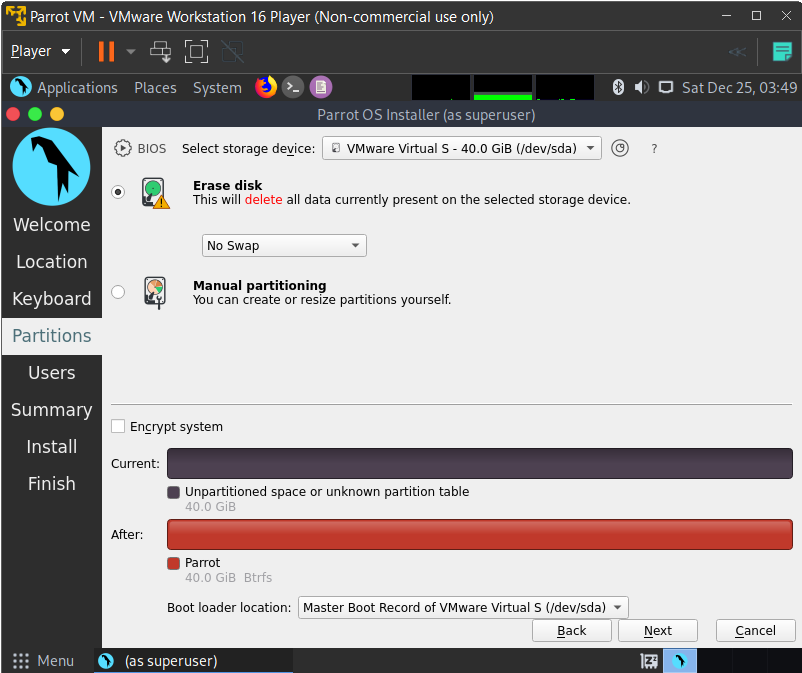
\includegraphics[width=0.75\textwidth]{Images/Install_OS/OS_6.png}
        \caption{Select "Erase disk" and press "Next".}
    \end{figure}

%___________________________________________________________________________________________________________  
    \clearpage
    \begin{figure}[h]
        \centering
        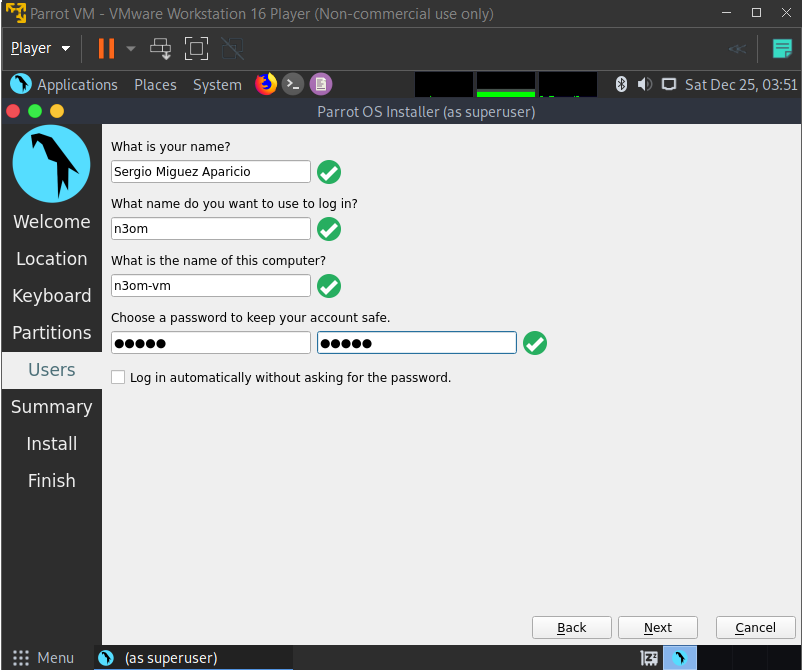
\includegraphics[width=0.73\textwidth]{Images/Install_OS/OS_7.png}
        \caption{Input your name, the username you want to use, the name of your system (it can be whatever
        you want), and add a strong password. Finally, press "Next".}
    \end{figure}

    \vfill

    \begin{figure}[h!]
        \centering
        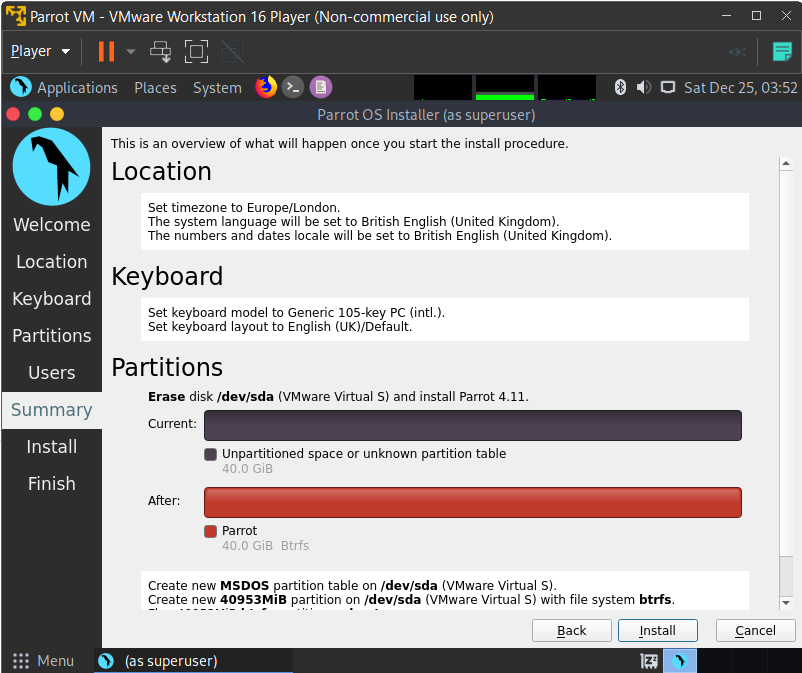
\includegraphics[width=0.73\textwidth]{Images/Install_OS/OS_8.png}
        \caption{A final Overview will be shown to the user. If everything is correct, press "Install".
        A warning will show up, press "Install now".}
    \end{figure}

%___________________________________________________________________________________________________________  
    \clearpage
    \begin{figure}[h]
        \centering
        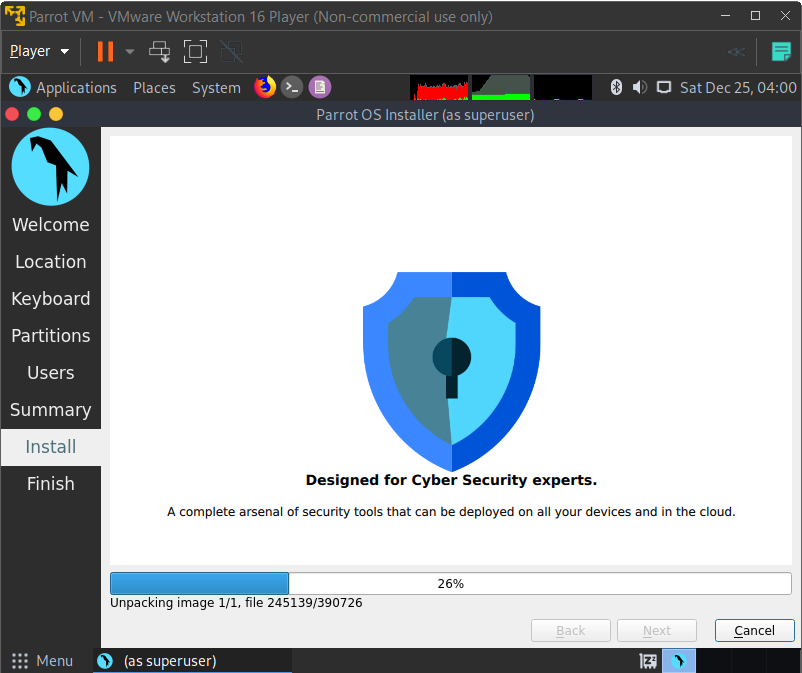
\includegraphics[width=0.74\textwidth]{Images/Install_OS/OS_9.png}
        \caption{The process will take a few minutes while the OS gets installed.}
    \end{figure}

    \vfill

    \begin{figure}[h!]
        \centering
        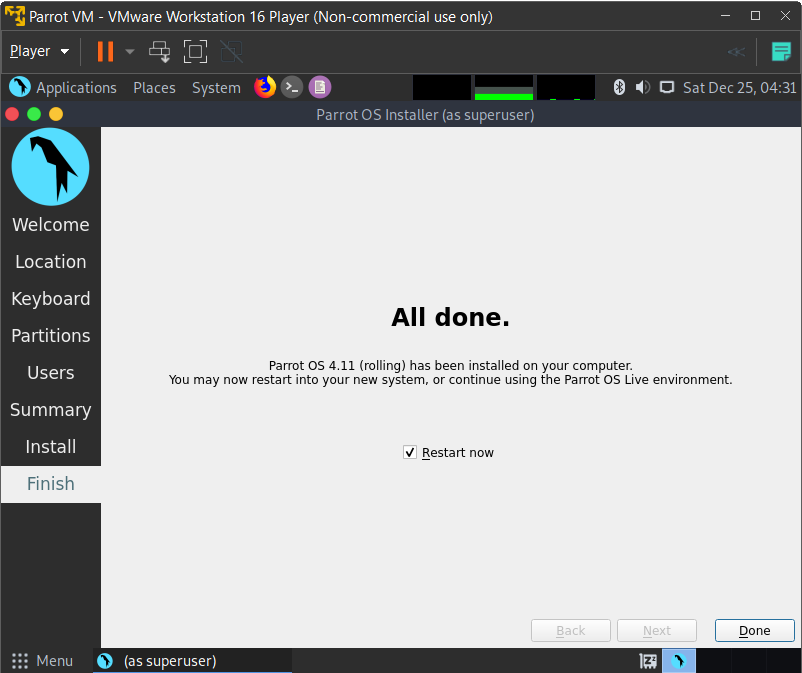
\includegraphics[width=0.74\textwidth]{Images/Install_OS/OS_10.png}
        \caption{When the installation is over, press "Done". Then press any key when it is requested and
        the system will boot completely.}
    \end{figure}

%___________________________________________________________________________________________________________  
    \clearpage
    \begin{figure}[h]
        \centering
        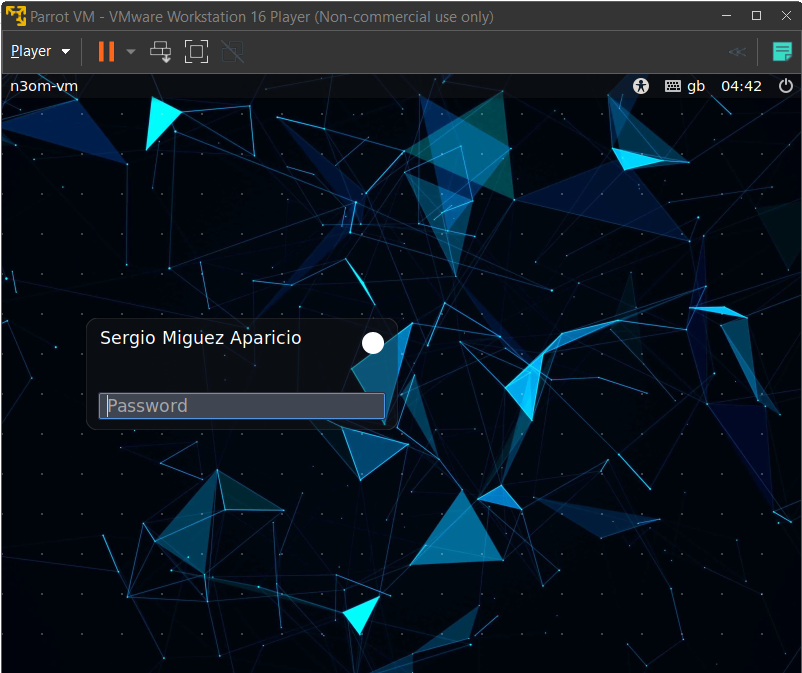
\includegraphics[width=0.75\textwidth]{Images/Install_OS/OS_11.png}
        \caption{Login into your new VM. The process is done.}
    \end{figure}

%___________________________________________________________________________________________________________  
    \clearpage
    \subsection{\textbf{Updating Parrot OS}}
    \begin{tcolorbox}[colback=red!25!white,colframe=red]
        \centering
        \textbf{It is REALLY IMPORTANT that you use the following process to update your Parrot Machine.}
    \end{tcolorbox}

    \tab Open the "MATE Terminal" clicking on Applications/System Tools/MATE Terminal as shown in the following
    figure:

    \begin{figure}[h]
        \centering
        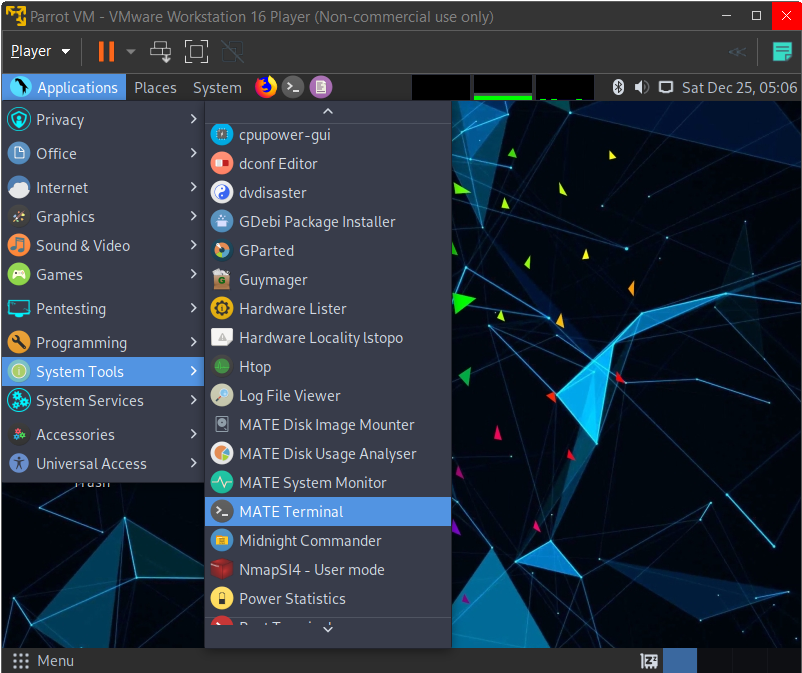
\includegraphics[width=0.63\textwidth, keepaspectratio]{Images/Updating_OS/Updating_1.png}
        \caption{Opening the Terminal.}
    \end{figure}

    \textbf{A faster option is to click directly on the MATE Terminal icon shown in the following figure:}

    \begin{figure}[h!]
        \centering
        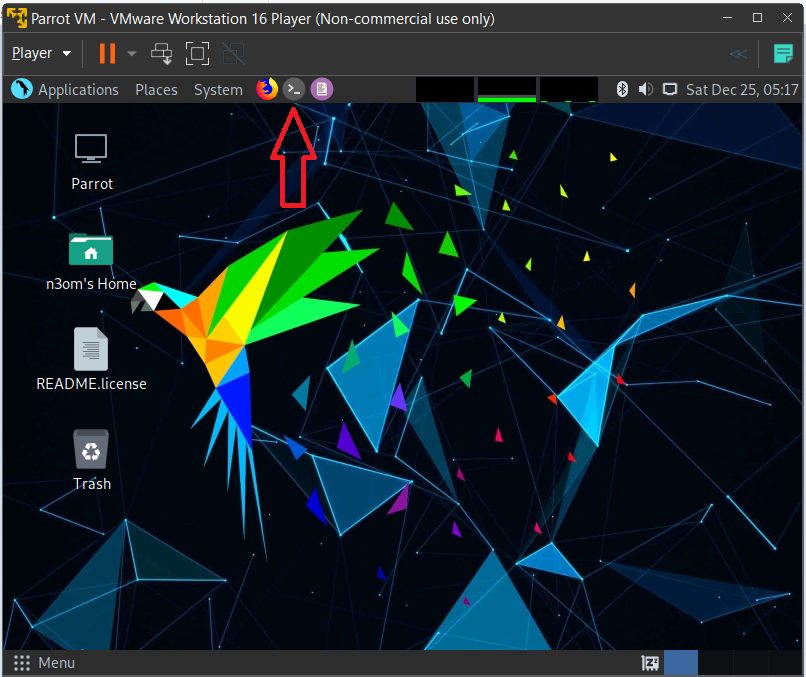
\includegraphics[width=0.63\textwidth, keepaspectratio]{Images/Updating_OS/Updating_2.png}
        \caption{Opening the Terminal Button.}
    \end{figure}

    \tab Having opened the terminal, enter the following code:

    \begin{lstlisting}[language=Bash, caption=Updating Parrot OS]
        sudo apt update
        # Enter your password
        sudo parrot-upgrade
    \end{lstlisting}

    \vspace{0.5cm}

    \begin{tcolorbox}[colback=red!25!white,colframe=red]
        \centering
        \textbf{It is REALLY IMPORTANT NOT to USE "sudo apt upgrade" as some packages which could be specifically 
        updated for this distribution would be overwritten to install the latest version.
        This could cause later on problems using or updating the system.}
    \end{tcolorbox}

    \vspace{0.5cm}

    \begin{tcolorbox}[colback=green!25!white,colframe=green]
        \centering
        \textbf{Use sudo parrot-upgrade}
    \end{tcolorbox}

    \vspace{0.5cm}

    \tab Wait while your system gets updated to the last version. It can take a few minutes.
    Finally, if the system requires it, use the following code to remove the unnecessary previous version files no longer in use.

    \begin{lstlisting}[language=Bash, caption=Removing deprecated files.]
        sudo apt autoremove -y
    \end{lstlisting}

%___________________________________________________________________________________________________________  
    \clearpage
    \section{Bibliography}
    \renewcommand{\sectionName}{Bibliography}

    \begin{enumerate}
        \item VMware - Last accessed on 26/12/2021 - \href{https://www.vmware.com/topics/glossary/content/virtual-machine.html}{\textcolor{blue}{https://www.vmware.com/topics/glossary/content/virtual-machine.html}}
        \item Oracle VirtualBox - Last accessed on 26/12/2021 - \href{https://www.virtualbox.org/manual/ch01.html}{\textcolor{blue}{https://www.virtualbox.org/manual/ch01.html}}
        \item Parrot OS - Last accessed on 26/12/2021 - \href{https://www.parrotsec.org/download/}{\textcolor{blue}{https://www.parrotsec.org/download/}}
    \end{enumerate}

\end{document}